
\documentclass[fontsize=12pt]{scrartcl} % A4 paper and 12pt font size

\usepackage[T1]{fontenc} % Use 8-bit encoding that has 256 glyphs
%\usepackage{fourier} % Use the Adobe Utopia font for the document - comment this line to return to the LaTeX default
\usepackage{spverbatim}
\usepackage[bottom=6em]{geometry}
\usepackage[english]{babel} % English language/hyphenation
\usepackage[babel=true]{csquotes} 
\usepackage{amsmath,amsfonts,amsthm} % Math packages
\usepackage{lipsum} % Used for inserting dummy 'Lorem ipsum' text into the template
\usepackage{graphicx}
\usepackage{titlepic} 
\usepackage{bbm}
\usepackage{color}
\usepackage{sectsty} % Allows customizing section commands
\usepackage{listings} %Allows Java code
\setlength{\headheight}{0pt} % Customize the height of the header





%\numberwithin{equation}{section} % Number equations within sections (i.e. 1.1, 1.2, 2.1, 2.2 instead of 1, 2, 3, 4)
%\numberwithin{figure}{section} % Number figures within sections (i.e. 1.1, 1.2, 2.1, 2.2 instead of 1, 2, 3, 4)
%\numberwithin{table}{section} % Number tables within sections (i.e. 1.1, 1.2, 2.1, 2.2 instead of 1, 2, 3, 4)


%----------------------------------------------------------------------------------------
%	TITLE SECTION
%----------------------------------------------------------------------------------------

\newcommand{\horrule}[1]{\rule{\linewidth}{#1}} % Create horizontal rule command with 1 argument of height
\title{	
 %  
\includegraphics[width=4cm]{lia-logo.jpg} % also works with logo.pdf
\normalfont \normalsize 
\textsc{Intelligent Agents, EPFL} \\ [20pt] % Your university, school and/or department name(s)
\horrule{0.5pt} \\[0.4cm] % Thin top horizontal rule
\huge Centralized agents \\ % The assignment title
\horrule{2pt} \\[0.5cm] % Thick bottom horizontal rule
}
\author{Jeremy Gotteland \& Quentin Praz} % Your name
\date{\normalsize\today} % Today's date or a custom date
\begin{document}
\maketitle % Print the title

%----------------------------------------------------------------------------------------
%	PROBLEMS SECTION
%----------------------------------------------------------------------------------------

\section*{Encoding the problem}
We create the class $ExtendedTask$ which is the extension of a basic task provided by \textit{Logist}. This new class is used to differentiate the pickup action and the delivery action. It is characterize by a task and by an action (pickup or delivery). We used these $ExtendedTask$s to be able to carry multiple tasks in the same vehicle.\\
We also implement the class $Solution$ which represents a possible solution. A solution is characterized by a map between a vehicle and a list of $ExtendedTask$s that we called $tasksList$. We have therefore one $tasksList$ per vehicle.\\
The notion of time is defined by the indices of the task in the $tasksList$.

\section*{Constraints}
To have a valid solution, we need to satisfy constraints:
\begin{enumerate}
\item A specific $ExtendedTask$ can be contained in only one $tasksList$.
\item Let take the two $ExtendedTask$s coming from the same task (pickup and delivery part), the index of the pickup part has to be strictly smaller that the index of the delivery part.
\item Let take again the two $ExtendedTask$s coming from the same task, the two $ExtendedTask$ have to be in the same $tasksList$.
\item All task must be delivered. The sum of the $ExtendedTask$s from all $tasksList$s had to be equal to the number of initial tasks multiplied by 2.
\item The weights of the carried tasks by a vehicle cannot exceed the capacity of this vehicle. 
\end{enumerate}

\section*{Generating the plans}

We use the \textbf{Stochastic Local Search} algorithm to determine the plan of each vehicle, leading to an optimal solution. This algorithm works iteratively: starting from an initial solution, each steps creates a new set of solutions based on the current chosen solution (neighbours) and selects the one that gives the best cost function. \\ \\

\subsection*{Local neighbours generation}

In order to perform the SLS algorithm, we need to generate a set of solutions that are similar to the one we are iterating on. \\

To generate neighbours, we first select a random vehicle which has at least one task to pickup/deliver. Then we apply to it the two following \textbf{operators}

\begin{itemize}
\item Swap task \textbf{between} vehicles: \\For every other vehicle, generate solution by replacing the two first actions of each vehicle by the pickup-delivery of the \textbf{first pickup of the other one}

\item Swap tasks \textbf{within} a vehicle: \\Generate as many solutions as there are possible combinations to swap \textbf{task order} within the random vehicle we chose.
\end{itemize}


From those we select the ones that are valid, and then compute their cost using the cost function described in the exercise sheet. \\
We select the solution that minimizes this objective function (if several solutions have the same value, we select one of them randomly). \\\\
Then comes into play a probability factor \textbf{p} that we set in the beginning \textbf{(here we chose the value 0.5)}. With probability \textbf{p}, we select the solution chosen before and continue SLS with this value as our current solution. But with probability \textbf{(1 - p)}, we stay in the same state and run again the algorithm, with the current state not being changed. \\\\
Note that we limit the number of iterations of SLS to \textbf{5000 iterations}.

\subsection*{The importance of the initial solution}
Our initial solution was to give task 1 to vehicle 1, task 2 to vehicle 2, etc.. . If we have 4 vehicles, we give task 5 to vehicle 1 (given that he has enough capacity) and we continue until all tasks are assigned. \\\\
This proved to converge to the right solution relatively quickly, as well as having a low computation time because the number of combinations of tasks within each vehicle was limited. \\\\
However, starting from an initial solution where all tasks were put in one vehicle gave much better result regarding to the cost, but had a much higher computation time. \\ \\
Result of the comparison are displayed in the \textbf{Results} section.


\section*{Results}

This graph contains all of our results. We ran the algorithm for 10, 20, 30 and 40 tasks, with everytime 1, 2, 3 or 4 vehicles. \\ \\
In the case of the initial solution where all tasks are put in one vehicle, they always stay in that same vehicles so we do not need to differentiate. \\\\
However it is important in the case where the initial solution tries to spread tasks in every vehicle.

\begin{figure}[h!]

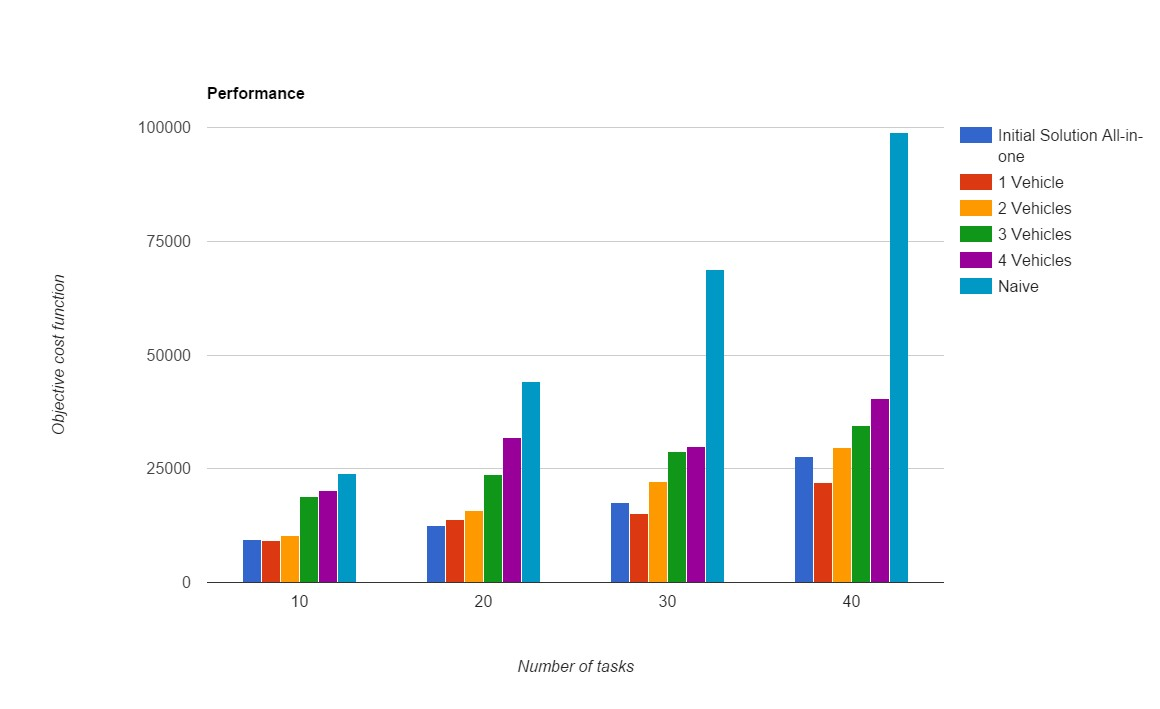
\includegraphics[width=\linewidth]{perf-graph.jpg}
\caption{Performance in terms of cost for each combinations of parameters/algorithm}

\end{figure}

\begin{table}
\centering
\begin{tabular}{|c|c|c|c|c|c|c|}
\hline
Number of tasks & All-in-one & 1 Vehicle & 2 Vehicles & 3 Vehicles & 4 Vehicles & Naive\\ 
\hline
10 & 9549 & 9196 & 10222 & 18890 & 20136 & 24029\\ 
\hline
20 & 12487 & 13855 & 15761 & 23732 & 31876.5 & 44214\\ 
\hline
30 & 17600 & 15241 & 22227 & 28739 & 29847 & 68731\\ 
\hline
40 & 27756 & 22027 & 29744 & 34488 & 40376.5 & 98896\\ 
\hline
\hline\end{tabular}
\label{table:table}
\caption{\small{Values of the barplot}} 
\end{table}



\end{document}          
